\documentclass[nooutcomes]{ximera}
\input{../preamble.tex}



\author{Elizabeth Miller}
%\license{Creative Commons 4.0 International License}



\title{Relations and Graphs: Relations}

\begin{document}

\begin{abstract}
We define relations and graph examples of relations. 
\end{abstract}
\maketitle

%\typeout{************************************************}
%\typeout{Relations}
%\typeout{************************************************}

%\subsection{Relations} 
In the last section, we discussed plotting points using the Cartesian coordinate system. While individual points can be useful, we often want to study collections of points.

\begin{definition}
A \dfn{relation} is a collection of points of the form $(x,y)$.  If the point $(x_0,y_0)$ is in the relation, then we say $x_0$ and $y_0$ are \dfn{related}.
\end{definition}

This might seem like a strange definition, but hopefully a few
examples will you see the relationship (pun intended!) between the
mathematical definitions of the words ``relation'' and ``related'' and the
way we often use these words in everyday speech.

\begin{MM}
What is this $(x_0,y_0)$ notation?  When we write $(x,y)$, we are usually talking about a generic point.  When we write $(x_0,y_0)$, we have a specific point in mind.  $x_0$ and $y_0$ essentially serve as placeholders for a point such as $(-1.5, 2)$ or $(0,5)$. We read $(x_0,y_0)$ as ``$x$ naught, $y$ naught."
\end{MM}

\begin{example}
Let's look at the relationship between the number of chicken nuggets
you can buy in a single container at a local fast food store and the
price in dollars for that container of nuggets.

$$
 \begin{array}{||c c||} 
 \hline
 \text{Number of Nuggets} & \text{Price (in dollars)} \\[0.5ex] 
 \hline\hline
 4 & 1.99\\ 
 \hline
 6 & 2.99 \\
 \hline
 10 & 4.49\\
 \hline
 20 & 5.00 \\
 \hline
 40 & 8.99\\[1ex] 
 \hline
\end{array}
$$

\begin{explanation}
This table defines a relation because we can list these as the points $(4,1.99)$, $(6,2.99)$, $(10,4.49)$, $(20,5.00)$, and $(40, 8.99)$.  We say that 4 nuggets is related to $\$1.99$ and $40$ nuggets is related to $\$8.99$.  We can also represent this relationship using a graph.

\begin{image}
\begin{tikzpicture}
    \begin{axis}[xlabel={nuggets},
                    ylabel={cost (in dollars)},
                    xmin=-1,xmax=45,
                    ymin=-1,ymax=10,
                    xtick={5,10,...,45},
                    minor xtick={5,10,...,45},
                    ytick={1,2,...,9},
                    minor ytick={1,2,...,9},
                    ]
        \addplot[soliddot] coordinates {(4, 1.99)} node[below] {$(4,1.99)$};
        \addplot[soliddot] coordinates {(6, 2.99)} node[above] {$(6,2.99)$};
        \addplot[soliddot] coordinates {(10, 4.49)} node[right] {$(10,4.49)$};
        \addplot[soliddot] coordinates {(20, 5)} node[above] {$(20,5.00)$};
        \addplot[soliddot] coordinates {(40, 8.99)} node[above] {$(40,8.99)$};
    \end{axis}
\end{tikzpicture}
\end{image}

We could ask many mathematical questions about this relation.  For example, ``What's the cheapest way to buy 100 nuggets?"  But for now, its enough to know it is a relation and to know you can represent that relation using multiple representations such as a table, a list, or a graph.
\end{explanation}
\end{example}

\begin{MM}
Representations are important in math. There are often many different ways information can be displayed or described. Common representations include tables, graphs, formulas, or drawings. Representations help us make sense of mathematics in different ways. Key for mathematical understanding is making connections between different representations and being able to move or `translate' between them.
\end{MM}



\begin{example}
It's important to note that nothing about our definition of relation
restricts what points can be included.  Assume that in our chicken
nugget example above, there is a coupon that allows you to buy $10$
chicken nuggets for $\$3.00$ and there an option to buy a chicken
nugget meal which includes $10$ chicken nuggets (and fries and a
drink) for $\$6.49$.

\begin{explanation}
We could modify the table of our relation to be:

$$
 \begin{array}{||c c||} 
 \hline
 \text{Number of Nuggets} & \text{Price} \\[0.5ex] 
 \hline\hline
 4 & 1.99\\ 
 \hline
 6 & 2.99 \\
 \hline
 10 & 4.49\\
 \hline
 20 & 5.00 \\
 \hline
 40 & 8.99\\ 
 \hline
 10 & 3 \\
 \hline
 10 & 6.49\\[1ex] 
 \hline
\end{array}
$$


This table still defines a relation and we can say that $10$ nuggets is
related to $\$4.49$ and $\$3.00$ and $\$6.49$. Here is the graph of
this relation.

\begin{image}
\begin{tikzpicture}
    \begin{axis}[xlabel={nuggets},
                    ylabel={cost (in dollars)},
                    xmin=-5,xmax=45,
                    ymin=-1,ymax=10,
                    xtick={5,10,...,45},
                    minor xtick={5,10,...,45},
                    ytick={1,2,...,9},
                    minor ytick={1,2,...,9},
                    ]
        \addplot[soliddot] coordinates {(4, 1.99)} node[below] {$(4,1.99)$};
        \addplot[soliddot] coordinates {(6, 2.99)} node[above] {$(6,2.99)$};
        \addplot[soliddot] coordinates {(10, 4.49)} node[right] {$(10,4.49)$};
        \addplot[soliddot] coordinates {(20, 5)} node[right] {$(20,5.00)$};
        \addplot[soliddot] coordinates {(40, 8.99)} node[above] {$(40,8.99)$};
        \addplot[soliddot] coordinates {(10, 3)} node[right] {$(10,3.00)$};
        \addplot[soliddot] coordinates {(10, 6.49)} node[above] {$(10,6.49)$};
    \end{axis}
\end{tikzpicture}
\end{image}
\end{explanation}
\end{example}


\begin{remark}
There is a special type of relation called a \textbf{function} where each $x$-coordinate is only allowed to be related to one unique $y$-coordinate.  The relation in example 1 is a function but the relation in example 2, which includes the coupon and a meal, is not a function because 10 nuggets is related to more than one cost.  Functions are going to be extremely important and we will come back to them later in the course.
\end{remark}

\begin{MM}
In example 2, we were given information (fries and drink) that wasn't used when describing the relation.  This type of `extra' information is usually present when using math to make decisons or answer questions in our every day life. One aspect of mathematics is determining what information to include or is relevant.
\end{MM}

The two examples we have seen so far have been a relations given by a list of points.  This does not have to be the case.  Relations can contain an infinite number of points.  Some of the relations we will focus on are given by an equation relating two variables.

\begin{example}
Let's consider the relation that is the collection of all points $(x,y)$ where $x^2+y^2=4$. 

\begin{explanation}
Some points contained in this relation are $(2,0)$, $(0,2)$, $(-2,0)$, and $(0,-2)$, but these are not all the points in this relation.  Often, one of best ways to think about a relation given by an equation is with a graph.  The graph of $x^2+y^2=4$ is the circle of radius 2 centered at the origin.

\begin{image}
\begin{tikzpicture}
    \begin{axis}[ymin=-3, ymax=3,
                         xmin=-3, xmax=3, 
                         axis equal]
        %\addplot[mark=none,domain=-2:2]{sqrt(4-x^2)};
        %\addplot[mark=none,domain=-2:2]{-sqrt(4-x^2)};
           %\draw (axis cs: 0,0) circle [radius=2];
          \addplot [domain=-180:180, samples=100] ({2*cos(x)},{2*sin(x)});
        \addplot[soliddot] coordinates {(0, 2)} node[above] {$(0,2)$};
        \addplot[soliddot] coordinates {(2, 0)} node[right] {$(2,0)$};
        \addplot[soliddot] coordinates {(0, -2)} node[below] {$(0,-2)$};
        \addplot[soliddot] coordinates {(-2, 0)} node[left] {$(-2,0)$};
    \end{axis}
\end{tikzpicture}
\end{image}

\end{explanation}
\end{example}

\begin{example} Verify algebraically that the point $(2,0)$ is on the curve $x^2+y^2=4$. 

\begin{explanation}
Note that this is the same question as, ``Verify that the point $(2,0)$ is a member of the relation given by $x^2+y^2=4."$  We want to show that this point satisfies the condition.
The point $(2,0)$ means that the $x=2$ and $y=0$.  If we plug these values in for $x$ and $y$ in the equation, we want to check that both sides of the equation are equal.
\begin{align*}
x^2+y^2&=4 \\
(2)^2+(0)^2&=4 \\
4+0 &= 4 \\
4 &= 4 
\end{align*}
\end{explanation}
\end{example}
\begin{example}
A relation can also be initially given by a graph.  For example, this is a relation.
\begin{image}
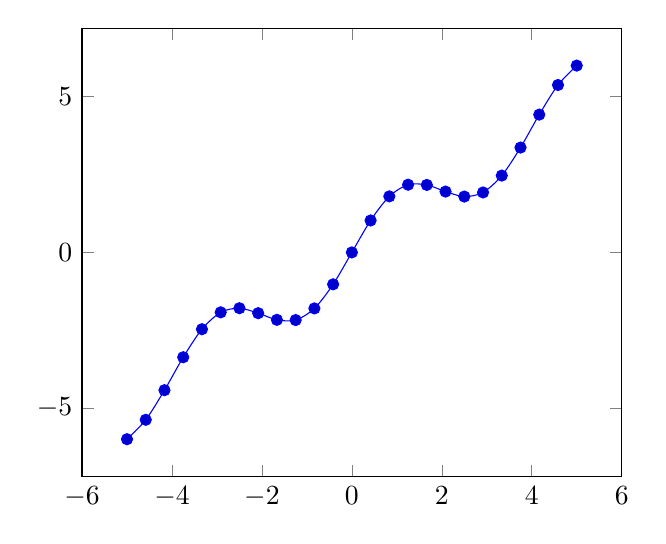
\begin{tikzpicture}
    \begin{axis}
        \addplot+[smooth] {x+sin(90*x)};
    \end{axis}
\end{tikzpicture}
\end{image}
\begin{explanation}
We can list some of the points on this graph.  It looks like $(0,0)$ and $(1,2)$ are points on this curve, but there are many other points we cannot explicitly list.
\end{explanation}
\end{example}
\end{document}
